\chapter{Introduction}\label{ch:intro}

% [SKELETON Habich restructure 2026-06-29] Lead-in for non-experts: from the general (search trees) to the
% specific (measurement system as the solution). Content from old kapitel/<lang>/01_introduction.tex, search-tree-first.

\section{Motivation}\label{sec:motivation}
Search trees and index structures form the foundation of modern data-intensive systems --- from in-memory
databases through file systems to language processing. At the same time, processors are dominated by the
memory hierarchy: not the number of operations but their cache behaviour determines the run
time~\cite{hennessy2019architecture, drepper2007memory, wulf1995memorywall}. From this tension arises
the guiding question of this thesis.
At its centre stand trie-based indexes and cache-line-optimized processing. Since the
Adaptive Radix Tree (ART)~\cite{leis2013art} of 2013, research has diversified: trie-height
optimization (HOT~\cite{binna2018hot}), hybrid B\textsuperscript{+} structures
(Masstree~\cite{mao2012masstree}, B\textsuperscript{2}-tree~\cite{schmeisser2022b2tree}),
hash/trie/B\textsuperscript{+} hybrid ordered indexes (Wormhole~\cite{wu2019wormhole}), succinct
representations (CoCo-Trie~\cite{boffa2024coco}, SuRF~\cite{zhang2018surf}), and self-tuning
approaches (START~\cite{fent2020start}).

\begin{figure}[htbp]\centering
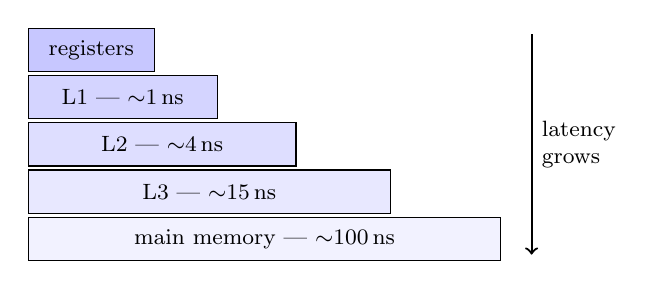
\begin{tikzpicture}[font=\footnotesize, lvl/.style={draw, minimum height=0.55cm, anchor=west, align=left}]
  \node[lvl, minimum width=1.6cm, fill=blue!22] at (0,2.0)  {registers};
  \node[lvl, minimum width=2.4cm, fill=blue!17] at (0,1.4)  {L1 --- $\sim$1\,ns};
  \node[lvl, minimum width=3.4cm, fill=blue!13] at (0,0.8)  {L2 --- $\sim$4\,ns};
  \node[lvl, minimum width=4.6cm, fill=blue!9]  at (0,0.2)  {L3 --- $\sim$15\,ns};
  \node[lvl, minimum width=6.0cm, fill=blue!5]  at (0,-0.4) {main memory --- $\sim$100\,ns};
  \draw[->,thick] (6.4,2.2) -- (6.4,-0.6) node[midway,right,align=left]{latency\\grows};
\end{tikzpicture}
\caption{The \enquote{cache wall}: typical orders of magnitude of the access latency per level of the
memory hierarchy (literature values after~\cite{hennessy2019architecture, drepper2007memory}); across the
hierarchy the latency grows by about two orders of magnitude.}\label{fig:cache-wall}
\end{figure}

In parallel, a research corpus of its own on cache awareness, prefetching, and allocation strategies
has emerged. Heuristics such as Cache-Sensitive Search Trees~\cite{rao1999css, rao2000csb},
cache-oblivious layouts~\cite{frigo1999cache}, prefetching B\textsuperscript{+}-trees~\cite{chen2001prefetch},
and hierarchical prefetching~\cite{zhang2025hierarchical} each address a separately considered aspect
of the search-algorithm architecture, with the focus mostly resting on empirically found improvements
and measurements. Because so much rests on cache-line-optimized behaviour, a segmentation of the
search-algorithm constituents into \emph{axes} suggests itself --- a backward-directed abstraction of
known building blocks into reusable modules across the most important works of the state of the art.

This thesis carries out this segmentation with a framework whose building blocks can be understood as
interchangeable design dimensions of a large \emph{design space}~\cite{idreos2018periodic, idreos2018datacalculator}.
Structurally different search methods --- from tree-like indexes to non-tree-like hash tables, including
special properties such as cache-line awareness --- thereby become comparable as points of the same
design space; non-tree-like methods occupy a restricted \emph{subset} of the dimensions over the same
search-algorithm interface, as if they formed the sole branch beneath the root. PRT-ART, a Probst
Redirect Tree / ART hybrid and an abstract, incomplete collection of novel search-algorithm
constituents, serves as the probe --- the candidate under test --- for state-of-the-art membership.

\section{Problem Statement}\label{sec:problem}
In today's search structures, cache awareness is either hard-wired or ignored entirely; above all, however,
one cannot \emph{separate} which individual design decision benefits which load pattern --- the
\emph{separability problem}, the central thread of this thesis.

Existing cache-aware index designs optimize one or a few aspects in isolation and report results that
are hard to compare across publications, because each work uses its own data structures, workloads, and
measurement methodology. The weightings of the improvements of individual algorithm constituents remain
inseparable: a reported performance gain cannot be unambiguously attributed to a single constituent
(page type, layout, value placement, prefetching), because the constituents stay intertwined in the
original designs. There is no common framework that (i)~decomposes such designs into interchangeable
axes, (ii)~reconstructs published algorithms as explicit configurations, and (iii)~can measure both
individual axes and whole algorithms on a uniform, fair basis.

\begin{figure}[htbp]\centering
\begin{tikzpicture}[font=\footnotesize, align=center, >=Stealth]
  \node[draw, fill=black!75, text=white, minimum width=2.4cm, minimum height=2.2cm] (mono) at (0,0){algorithm\\(monolith)\\[1mm]{\Large ?}};
  \node[font=\scriptsize] at (0,-1.65){which part helps?};
  \draw[->,very thick] (1.5,0) -- (2.9,0);
  \node[draw, fill=green!12, minimum width=2.2cm] (a1) at (4.9,0.85){node type};
  \node[draw, fill=green!12, minimum width=2.2cm] (a2) at (4.9,0.0){layout};
  \node[draw, fill=green!12, minimum width=2.2cm] (a3) at (4.9,-0.85){allocator};
  \node[font=\scriptsize] at (4.9,-1.65){each axis measurable in isolation};
\end{tikzpicture}
\caption{The separability problem: as a monolith it remains unclear which design decision takes effect; only the decomposition into orthogonal axes makes each contribution measurable in isolation.}\label{fig:separability}
\end{figure}

\section{Research Questions}\label{sec:rqs}
The task description and the goal of cache-line optimization give rise --- owing to the
ubiquity of the influence of the cache-line settings --- to one main question (RQ0) and four
measurable research questions (RQ1--RQ4); complementary aspects are assigned to them as deepening \emph{sub-questions}.
Across all five questions lies a categorization question that this thesis carries along as a coinage
of terms: the task description already distinguishes what is measured (the design constituents of the
algorithm), the platform on which building and measuring take place, and the measuring itself. Whether the
axes of the design space can be cleanly separated along these three concerns into \emph{organ axes} (the
interchangeable design constituents of the algorithm), \emph{system axes} (the concerns of the build
and target platform), and \emph{measurement axes} (the concerns of measuring itself) --- and
how such a separation is to be accomplished if a design does not yet provide
it --- is laid out as a question in this thesis; the sub-questions are therefore named along these three
\emph{axis categories}. The current state here is unambiguous: the thesis lays out the triad as
three separate axis registries\footnote{An axis registry is the directory of the axes of one
  category together with the building blocks offered per axis (in code a Registry).} --- an
organ-axis registry, a system-axis registry, and a
measurement-axis registry --- and tests their viability; the answers are developed by
Chapters~\ref{ch:measurement},~\ref{ch:impl}, and~\ref{ch:eval}.
Each question is thereby answered at exactly one place: RQ1 in Section~\ref{sec:axis-triad} and
Chapter~\ref{ch:impl}, RQ2 in Section~\ref{sec:measurement-system} and Chapter~\ref{ch:eval}
(RQ2.d in Section~\ref{sec:workload-basics-known} and Section~\ref{sec:eval-workloads}), RQ3 in
Section~\ref{sec:prtart-demo} and Chapter~\ref{ch:eval}, RQ4 in
Section~\ref{sec:impl-system-axes} and Section~\ref{sec:impl-pipeline} (RQ4.a);
Chapter~\ref{ch:conclusion} draws the balance per main question and
sub-question. For this, the sub-questions carry the identifiers RQ0.E, RQ1.a, RQ1.b, RQ2.a, RQ2.b, RQ2.c, RQ2.d,
RQ3.a, RQ3.b, RQ4.a, and RQ4.E.
\begin{description}
  %% OWNER-VORLAGE: OV-K1-01 --- the bracket expression \enquote{(hybrid CPUs, Sapphire Rapids)} is
  %% frozen Owner wording of the research question (scope freeze). It remains unchanged; the
  %% footnote carries the actual state of the measured fleet. Objection suffices.
  \item[RQ0 (Main question)] By how much do \emph{active, measurement-driven}\footnote{A decision is
  called measurement-driven when it is grounded in collected measured values and not in fixed model
  assumptions; a variant is statically dimensioned when its decision is fixed in advance at design time.}
  cache-aware
  decisions --- page type, memory layout, value placement, and prefetching --- improve the performance of
  trie-based search structures over \emph{passive, statically dimensioned} variants on
  different CPU platforms (hybrid CPUs, Sapphire
  Rapids)?\footnote{The measured fleet of this thesis consists of the three registered
  machine signatures: prod1 (AMD Zen~5, Ryzen~9~9950X3D), prod2 (Intel Core i9-12900K, Alder Lake --- % chktex 29
  a hybrid CPU with P and E cores), and an ODROID board with Intel Gracemont cores. The
  server platform Sapphire
  Rapids (ZIH node Barnard, Xeon~8470) is provided for in the platform detection but is not part of the
  measurement series (n/a).}
  \emph{Extension RQ0.E (axis categories):} Can a measured gain be attributed unambiguously at all
  --- to the design decision itself (organ), to the build and target platform (system), or to
  the measurement setup (measurement) ---, and which separation of the axis categories is necessary for this?
  \item[RQ1 (Composition)] How can a search-algorithm design be canonically decomposed into orthogonal
  axes and systematized in a permutation matrix\footnote{The decomposition is called canonical when every
  axis has a fixed place in a binding order. The permutation matrix is the
  table of these axes with their admissible assignments; each choice of exactly one assignment per axis is
  an axis permutation, and a profile is the declarative description (as XML) of a design
  by its assignment of these axes. Bias-free means: without distortion by a re-implementation
  or by unequal measurement conditions.} such that the
  state-of-the-art methods become reconstructable bias-free as profiles --- as far as possible from
  their original code --- and arbitrarily permutable? \emph{Sub-question RQ1.a (category cut):} Does
  the canonical decomposition itself divide along the three axis categories --- must platform and
  measurement concerns be kept out of the permutation matrix so that the decomposition of the
  design constituents remains orthogonal ---, and how is such a cut to be accomplished
  if it is not yet laid out in the design? \emph{Sub-question RQ1.b (organ couplings and
  system variation):} Which mutual dependencies between axes (node type $\times$ SIMD
  $\times$ path compression)\footnote{SIMD (\emph{single instruction, multiple data}) denotes
  instructions that apply one operation to several data elements at once; path compression merges,
  in a trie, node sequences without branching into one node; the ISA (\emph{instruction
  set architecture}) is the instruction set of the target CPU, and SSE2/AVX2/AVX-512, NEON/SVE2, and RVV are
  the SIMD extensions of the instruction sets x86, ARM, and RISC-V\@.}
  limit the isolation of individual axes, and how does the same organ assignment behave
  in its cache-update and cache-line fill behaviour (how the cache is updated and how completely
  the loaded cache lines are used) when the ISA/SIMD axis alone (SSE2/AVX2/AVX-512,
  NEON/SVE2, RVV) is varied --- as far as the respective target platform is released for building
  (Section~\ref{sec:axis-triad})?
  \item[RQ2 (Measurement methodology)] How must a reproducible measurement pipeline with
  hardware-counter collection\footnote{The measurement pipeline is the chain of building the binaries, measurement run,
  and evaluation; hardware counters are the performance counters of the CPU (\emph{performance monitoring
  counters}, PMC), which count events such as cache misses per run.} be designed so that every
  axis permutation is measured fairly (all else being equal,
  that is, on an identical compiler and flag basis) in three measurement series --- A (probe vs.\ state of the
  art), B (systematic variation of the design decisions), and C (merge/regression
  old vs.\ new) --- over three granularities (micro-, macro-, and overall benchmarking: individual
  constituents, interface operations, whole algorithms), and under which
  platform-calibrated criteria (thresholds that are determined per machine signature from measurement runs on the
  respective platform) does a platform count as successfully verified?
  \emph{Sub-question RQ2.a (measurement axes):} Must the measurement instruments themselves --- timing,
  counter collection, load generation --- be carried as axes of their own that are always present
  without ever changing what is built and measured, and how is this separation to be
  accomplished if it does not yet exist?
  \emph{Sub-question RQ2.b (organ axes):} How can contradictory findings in the literature on the optimal
  node/cache-line size (one cache line for CSS/CSB\textsuperscript{+}~\cite{rao1999css, rao2000csb}
  versus sixteen and more for Hankins/Patel~\cite{hankins2003nodesize}, there nodes of 512 bytes and
  larger at 32-byte cache lines, as well as several cache lines per node loaded jointly via prefetch
  in the prefetching B\textsuperscript{+}-trees of Chen, Gibbons, and Mowry~\cite{chen2001prefetch})
  be re-measured bias-free through axis-isolated measurement
  permuted with all else being equal,
  instead of being adopted from incompatible original setups?
  \emph{Sub-question RQ2.c (extensibility):} How extensible is such a measurement pipeline --- how do
  new probes and their design constituents integrate, how are they abstracted, and do they
  join existing families\footnote{In this thesis, family denotes the topmost
  division of the algorithms by their externally visible interface (such as \texttt{Map} or
  \texttt{Container}); each family carries its own subclasses with a fixed axis set.},
  found new families or a
  hybrid form; at which conceptual level should this cut run? Central here is:
  what constitutes an extension of the system in the first place, and how does adding or
  cutting away individual design constituents --- such as those originating from a single
  publication --- affect the attainable degree of cache-line awareness of the
  overall system? Does this require
  an operating mode that offers the design constituents of a selectable reference design from the
  literature in isolation as a closed axis set, in order to measure exactly this one publication
  --- with measurement and system axes remaining free-standing --- faithfully to the original?
  \emph{Sub-question RQ2.d (workload state of the art):} Which workloads belong to the state of the art
  specifically for search algorithms?
  \item[RQ3 (Probe comparison)] Does the probe PRT-ART win against the eight Rank-1 designs
  of the state of the art (SOTA for short; ART, HOT, Masstree, CoCo-Trie, START,
  B\textsuperscript{2}-tree, Wormhole,
  SuRF)\footnote{The \emph{ranks} order the state-of-the-art publications by centrality for this thesis: Rank-1 comprises the ten most important core works --- among them the eight standalone search designs as well as ARTSync (P08)~\cite{leis2016olc} and LOUDS (P09)~\cite{jacobson1989louds}, which enter as organs ---, Rank-2 the cache-aware layout and B\textsuperscript{+} precursors, and Rank-3 the prefetching, synchronization, and TU-Dresden hardware works.}
  and the Rank-2/3 SOTA \emph{not} through asymptotic novelty but through better
  microarchitectural properties\footnote{Cache-line utilization is the share of the bytes of a loaded
  cache line that are used; LLC is the last-level cache, the last cache level before
  main memory; the dTLB (\emph{data translation lookaside buffer}) buffers address translations for
  data accesses; a miss is a failed access that has to resort to the next, slower level; branch cost
  is the cost of jump instructions, above all of mispredicted branches.} --- higher
  cache-line utilization, fewer LLC and dTLB misses, lower branch cost, smaller hot
  search paths (the frequently traversed node sequences) --- for exact lookup, prefix lookup (search for
  a key prefix), and prefix enumeration (enumeration of all keys for a prefix),
  measured under the three mandatory measurement series A (probe vs.\ state of the
  art), B (systematic variation of the design decisions), and C (merge/regression old vs.\
  new)? \emph{Sub-question RQ3.a (organ axes):} Which local page representation (8-/16-bit array-indexed page ---
  the direct-index pages Array$_{256}$ and Array$_{65535}$ --- versus the vector page --- the
  vector pages Vector$\langle$u8,u8$\rangle$ and Vector$\langle$u16,u16$\rangle$) is cheapest per
  branch point (per node at which the search path branches), and by which
  platform-calibrated
  switching rules --- including the order
  Array$_{256}\to$Array$_{65535}\to$Vector$\langle$u8,u8$\rangle\to$Vector$\langle$u16,u16$\rangle$
  by occupancy density and access type --- should switching occur adaptively? The probe currently switches by fixed
  density thresholds of 25, 50, and 75~percent\footnote{Array-indexed page and vector page are the two
  page forms of the PRT-ART B\textsuperscript{+} node: the array-indexed page addresses entries directly via an array with an 8-
  or 16-bit index, the vector page holds sorted key-value vectors. The density thresholds
  are the probe's switching rules between the page representations; the 50~percent boundary named in the
  glossary is the page-type boundary between array-indexed and vector page, not a further
  switching rule.} (Section~\ref{sec:prtart-demo}).
  \emph{Sub-question RQ3.b (compile-time force):} Do latency-critical measurements force decisions that are
  in principle selectable at run time --- such as those adaptive switching rules --- to be
  fixed as requirements already at compile time, so that every axis divides into a
  compile-time-fixed main axis and run-time-variable sub-axes
  --- a sharpening that RQ4 takes up?
  \item[RQ4 (Compile time vs.\ run time)] Which axis properties must be fixed at compile time
  in order to produce platform-optimized, provenance-verifiable\footnote{Provenance-verifiable
  means: the origin of a binary --- which axis assignment, which platform, and which
  toolchain brought it forth --- is verifiable on the binary itself. For this, every
  binary carries two identities: the binary identity per permutation, that is, its assignment of the organ axes
  (in code the \texttt{binary\_id}, a path of one segment per axis with a bijective
  numeric encoding), and the compile-time identity, which additionally comprises build platform, toolchain,
  build control quantities, and source state and is compiled into the binary as a fingerprint --- a hash over all
  build-determining members ---; the first is also called the
  permutation identity.} binaries per permutation, and which can or must be selected at run time
  (bit-encoded binary identity per permutation, run-time-adaptive layout selection) without violating
  scientific comparability (identical compiler and flag basis)? Does the measurement make it possible to
  generate ISA+OS-optimized binaries for a search-algorithm recombination whose heuristic
  optimization is perfectly tailored to its runtime environment?
  \emph{Sub-question RQ4.a (declarative chain):} Can the entire process --- from the platform-specific
  build of all binary permutations of the design constituents through the measurement run and the selection of the best
  measured binary or binary recombination to the evaluation in CSV/xlsx files, LaTeX, and
  diagrams --- be generated throughout from one XML description of the experiment, such that an
  experiment is completely and reproducibly determined by its declaration?
  \emph{Extension RQ4.E (system axes):} Does the boundary between compile time and run time run
  along the axis categories --- do the platform properties in particular (ISA,
  operating system, extension hardware such as GPU, FPGA, or NPU accelerators) belong, as system concerns, to
  the compile-time identity of the
  binary --- that is, to its fingerprint, without changing the permutation identity ---, while
  measurement choices (the assignments of the measurement axes) may remain run-time-variable?
\end{description}

\section{Objective and Contributions}\label{sec:contributions}
The objective follows the task description in four steps: decompose cache-aware search algorithms into
interchangeable design constituents, reconstruct state-of-the-art designs as explicit configurations,
measure and evaluate cache-line-aware behaviour both per constituent and for the whole algorithm
on a common CPU-only basis, and deliver the best overall algorithm --- following an autonomous
heuristic-profile evaluation and heuristic-function modelling --- as a standalone binary.
The code of the diploma thesis is here the \emph{formal consumer and driver} of the cache engine: it loads the
probe PRT-ART, compiles it via metaprogramming against the core constituents of the cache engine, delivers
ABI-stable \emph{living beings} (search-algorithm instances), and drives them to measurement via the probe dock --- the
measurement interface of the family (Chapter~\ref{ch:measurement}).
The underlying architecture model
--- the three levels (\emph{family} as the outer algorithm interface, \emph{genus} as the family subclass with a
fixed axis set, in code the tier subclass\footnote{\emph{Tier} is the German word for \emph{animal}: in the
  metaphor canon of this thesis it names the fully composed module --- the living being with all its
  organs (see \emph{Tier binary} in the glossary) ---, not a level or layer.} \texttt{AnatomyGenus}, and the
axis organs), the four subsystems, and the ABI-stable delivery of the search-algorithm \emph{living beings}
--- is developed by
Chapter~\ref{ch:measurement} and Chapter~\ref{ch:impl}. Meant here are the four carrier subsystems
measurement driver, \texttt{CacheEngineBuilder}, \texttt{CacheEngine}, and probe; to be distinguished from them are
the twelve stages of the recommendation pipeline in code. The concept of the axis architecture itself is adopted from
prior work by the author --- the axis concept of this predecessor implementation UltiHash (on its origin see
Section~\ref{sec:anatomy-patterns}) ---; the contribution of this thesis is
its transfer to cache-aware search structures and its measurement-oriented realization. The
central contributions are:
\begin{itemize}
  \item An ABI-stable module interface: a uniform C module boundary exports exactly one living being
  per permutation (\texttt{comdare\_\allowbreak{}create\_anatomy()} $\to$ \texttt{IAnatomyBase}); behind it
  lies a three-layer abstraction chain --- a
  mediating facade (\texttt{ICacheEngine}) above the runtime ABI layer
  (\texttt{IAnatomyBase} $\to$ \texttt{IExecutionEngine}) above the axis organs. The delimitation of the
  search-engine module is conceptually fixed but not implemented as a module of its own; its
  provider is expressly deferred, and the search-engine module is realized as a
  topic namespace within the cache engine. The probe's search core specializes its hybrid API variadically by
  parameter count (1~parameter $\Rightarrow$ \texttt{std::vector} API\@;
  2~parameters $\Rightarrow$ \texttt{std::map} API\@; $N>2 \Rightarrow$
  \texttt{std::map<K,\,std::tuple<V$_1$\ldots V$_N$>>}), as the task description demands across all variants
  of the well-known \texttt{std::map} and \texttt{std::vector} container hulls; for this, the cache engine
  provides the family arities of its genera.
  \item An axis permutation matrix in a three-part order: eighteen organ main axes in fixed
  slot order (T00--T17) form the binary permutation; three system main axes --- target ISA,
  operating system, and extension hardware --- describe the build and target platform, whereby their
  complex bracket \texttt{build\_target\_complex} is expressly not a fourth main axis; and a
  separate measurement-axis realm keeps the measurement concerns apart from both, for neither system nor
  measurement axes ever enter the permutation identity of the binary. An optional nineteenth
  organ axis for disk input/output, which does not describe an assignment but describes how other
  axes are described, is added as soon as disk input/output is integrated into the algorithm design;
  it stamps in the bracket appendage of the organ line and remains outside the
  permutation identity. The matrix is realized with Boost.MP11 compile-time type-list building blocks ---
  runtime tags and \texttt{std::variant} are excluded in the tier binaries as a principle of this thesis
  (\texttt{[[no-runtime-switch]]}) --- together with a compile-time fallback between the probe stack and the
  state-of-the-art stack, which takes over sixteen of the eighteen axes from the cache-engine frame and
  replaces two by probe slots.
  \item Thirty-three state-of-the-art profiles as persisted XML configurations (P01--P33):
  30~full profiles of standalone search designs --- 8~Rank-1 and 22~Rank-2/3 --- as well as 3~abstract profiles
  (OLC, LOUDS, VAMPIR), which enter only dissected, as organs or as measurement technology. The
  \texttt{ExperimentDriver} transforms them automatically into pre-compiled C++23 modules; the profile set
  thereby covers all 33 analysed publications. By means of the
  cache engine, the XML design genuinely maps the individual algorithm constituents at compile time and is thereby a
  compiler-compiler build recipe within a \emph{model-driven} optimization
  stack~\cite{schmidt2006modeldriven}; that declarative configuration descriptions drive the
  automated construction of modular system variants is an established
  construct~\cite{czarnecki2000generative, apel2013feature}.
  \item PRT-ART as a probe with eight building-block layers of its own (4+1+2 pool allocator, optimistic
  lock coupling with reserved blocks, MultiLevel layout, path-oriented prefetch,
  DensityTracker, hypothesis metrics H1/H2/H3, Inline/External/ChainRef value handles,
  signalling-bit serialization). In the measurement apparatus the probe registers four probe slots --- page type
  (\texttt{page\_type}, in the cache engine the axis \texttt{node\_type}), prefetch, telemetry, and the
  ChainRef value handle --- as well as a merge organ for path compression, which contains the cache engine's own
  Patricia strategy; in the codegen-capable measurement path two of them take effect (prefetch and
  value handle), while MultiLevel layout, pool allocator, and serialization run via the
  cache-engine default (Section~\ref{sec:prtart-demo}). In the cache engine, telemetry is
  a system axis and not a composition slot; the probe slot of the same name is a
  remaining holdover. The OLC concurrency is a building-block layer of the probe, not a registered slot.
  Note that the slot numbers of the probe do not follow the slot order T00--T17 of the
  cache engine. The deployment of the probe demonstrates the extensibility of the system by example ---
  towards the efficient advancement of novel approaches in dealing with cache-aware algorithms and
  accelerated search.
  \item A measurement driver with a defined-/full-mode distinction (supplemented by a deterministically
  sampled full variant), profile-aware workload routing --- by default the full permutation over all registered workloads, whose implementation status
  Chapter~\ref{ch:eval} reports --- and three granularities: micro-, macro-, and overall benchmarking
  (individual constituents, interface operations, whole algorithms).
  \item A build and measurement chain behind this driver that is declaratively controlled throughout: an
  experiment \emph{planner} resolves the XML description of the experiment against the axis offerings of the
  three axis registries, and the \texttt{CacheEngineBuilder} builds and measures from it
  the binary permutations per platform --- up to the evaluation via the xlsx output (the workbook
  is the output and the standard; the CSV form is not a single child document but an ordered tree of
  CSV files --- one overall folder per workbook, beneath it one folder per sheet, therein the CSV files of the
  individual sub-axis sweeps ---, which is always generated from the workbook, as a strategy of the same factory,
  and by XML lies at the same target instead of the workbook or in addition to it) and the
  LaTeX tables and TikZ diagrams generated from it.
  \item A bias-free comparison matrix that runs \emph{all} registered load profiles against \emph{all}
  reconstructed living beings --- the original-design binaries built from the profile XML --- and
  thereby counters the self-favouring through author-owned measurement setups in individual publications
  (pattern term: \emph{home-field advantage})~\cite{vanderkouwe2019benchmarking}.
  \item A generic platform probe that determines the cache properties per target platform ---
  line size and the sizes per hierarchy level from sysfs and CPUID --- and lets them flow as fixed quantities into a
  system-optimized binary. The core topology (P-/E-core separation, pinning) is envisaged as a
  platform concern of the same probe and is mandatory for the cache-line measurement on hybrid CPUs,
  but its capture by the probe is not implemented --- the implementation status is stated in
  Chapter~\ref{ch:eval}. The measurement plan provides for two operating-system regimes on the two production machines
  (immutable Talos and root Linux with full hardware-counter access); measured is the
  root-Linux regime, not the Talos regime.
  \item \emph{As objective and outlook:} the delivery and substantiated evaluation of the best
  overall algorithm --- automatically selected from the fine-grained measurement results under the
  measurement aspect of the best cache-aware behaviour and of the acceleration through cache-line adaptation, in
  comparison of all measurable parameters against the binary competitors --- as a standalone, ABI-stable
  binary behind the uniform search-algorithm interface. The measurement pipeline already delivers the
  ranking required for this, and a first increment of the automatic selection and of the
  binary delivery is implemented as a standalone tool (\texttt{best\_binary\_selector});
  the heuristics-driven full automation remains outlook.
\end{itemize}

\section{Structure of the Thesis}\label{sec:structure}
The structure follows the path from the general to the specific: Chapter~\ref{ch:foundations} lays --- conceptually
and visually --- the foundations from established knowledge: the landscape of search structures, the
hardware properties of the memory hierarchy, the workload conventions of the comparison literature, the
software means of abstraction, and the notion of a heuristic. Chapter~\ref{ch:measurement} develops
from them the concepts of a cache-aware measurement system: the problem statement and its
requirements, the state of the art as axis instances, the anatomy model with its layers, the
measurement system itself, the probe PRT-ART as demonstrator, and the heuristic evaluation
with its operating modes. Chapter~\ref{ch:impl} realizes this concept as a software architecture ---
repositories, the probe in code, the axis architecture and compilation pipeline, layer
contracts with contract tests, and the system axes in code. Chapter~\ref{ch:eval} evaluates along the
research questions, including the heuristic counter-evidence; Chapter~\ref{ch:conclusion} closes with
conclusion and outlook. The appendices deepen alongside: the measurement-series documentation
(Appendix~\ref{app:measurements}), the code structure (Appendix~\ref{app:code}), the glossary
(Appendix~\ref{app:glossary}), the complete building-block matrix (Appendix~\ref{app:blocks}), the
architecture decisions (Appendix~\ref{app:adr}), and the comparison interfaces
(Appendix~\ref{app:interfaces}).
